\documentclass[11pt]{extarticle}

% meta
\title{Отчет о лабораторной работе №3 \\[6mm] \large Обработка и распознавание изображений, ММП ВМК МГУ.}
\author{Аристархов Данила Дмитриевич.}
\date{Май 2024.}

\usepackage[warn]{mathtext}
\usepackage[T2A]{fontenc}			% кодировка
\usepackage[utf8]{inputenc}			% кодировка исходного текста
\usepackage[english,russian]{babel}	% локализация и переносы
\usepackage{indentfirst}
\usepackage{csquotes}
\usepackage{svg}
\usepackage{wrapfig}
\usepackage{listings}
% \usepackage[bibstyle=gost-numeric, sorting=none]{biblatex}
% \addbibresource{biblio.bib}

% page settings
\usepackage[
    left=1.8cm,
    right=1.8cm,
    top=1.8cm,
    bottom=1.8cm,
    bindingoffset=0cm
]{geometry}

\usepackage{graphicx, hyperref, xcolor}
\hypersetup{
    colorlinks=true,
    linkcolor=blue,
    filecolor=magenta, 
    urlcolor=blue,
    citecolor=blue,
    pdftitle={GD},
    % pdfpagemode=FullScreen,
    linktoc=all
    }

\usepackage{wrapfig,caption}

% figures
\usepackage{caption}
\usepackage{subcaption}
\usepackage{floatrow}
\floatsetup{heightadjust=object}

\graphicspath{{img}}

% math
\usepackage{amsmath,amsfonts,amssymb,amsthm,mathtools,esint,eucal}

\begin{document}

\maketitle
{
  \hypersetup{linkcolor=black}
  \tableofcontents
}
\newpage

\section{Постановка задачи}
Необходимо разработать и реализовать программу для работы с изображениями для классификации изображений моделей графов,
построенных из магнитной головоломки. Программа должна производить сегментацию изображения, генерацию признаковых описаний структуры графов и классификацию изображения в соответствии с заданным набором эталонов. Также необходимо разработать пользовательский интерфейс для работы с программой, обеспечивающий выбор изображения, выполнение операций преобразования и выдачу результата.

\section{Описание данных}
Данные представляют из себя растровые изображения, на которых изображены модели графа, построенных из деталей магнитной игры-головоломки.

\begin{figure}[h]
  \centering
  \includesvg[width=\textwidth]{channels.svg}
  \caption{Разложение изображения по параметрам HSV}
  \label{fig:channels}
\end{figure}

\section{Описание метода решения}
\subsection{Сегментация изображения}
Первым этапом алгоритма является выделение маски ребер графа.

\begin{enumerate}
  \item Сначала изображение переводится в HSV (Hue, Saturation, Value) представление. В таком формате проще сегментировать изображение.
  \item Далее проводится бинаризация изображение по HSV параметрам. Данные параметры подбирались путем анализа изображений по отдельным компонентам (см. \autoref{fig:channels}), а также путем экспериментов. Оптимальные значения могут отличаться в зависимости от изображения. Для данной задачи были выбраны следующие пороги:
  \begin{enumerate}
    \item Изображения на белом фоне:
    \begin{enumerate}
      \item Hue $\in [50, 140]$
      \item Saturation $\in [0, 255]$
      \item Value $\in [150, 255]$
    \end{enumerate}
    \item Изображения на пестром фоне:
    \begin{enumerate}
      \item Hue $\in [30, 100]$
      \item Saturation $\in [30, 255]$
      \item Value $\in [0, 255]$
    \end{enumerate}
  \end{enumerate}
  \textit{Замечание:} Все параметры HSV были приведены к значениям $[0, 255]$.
  \item Для удаления шумов использовался медианный фильтр с ядром $(7, 7)$.
  \item Также используется открытие с ядром $(7, 7)$.
\end{enumerate}

\subsection{Построения скелета изображения}
Далее по полученной маске строится скелет изображения. Из маски удаляются связные компоненты размером менее заданного порога. Данный параметр выбирается в зависимости от изображения и определяет чувствительность алгоритма к шумам. Для данной задачи порог был выбран равным 20 пикселям. Таким образом, удается получить отрезки толщиной в один пиксель, являющимися очертаниями ребер графа. 

\subsection{Построение признакового описания структуры графа}
В качестве признакового описания графа был выбран вектор в котором, $k$-я компонента есть число вершин степени $k$ в представленном графе.
Построение этого вектора происходит в 2 этапа.
\begin{enumerate}
  \item Выделение концов отрезков, соответствующим ребрам. Для этого выделяются пиксели, у которых в окрестности $(3, 3)$ присутствуют ровно 2 пикселя (включая сам этот пиксель). Этим пискелям как раз и соответвуют концы отрезка.
  \item Подсчет степеней вершин. Для этого концы отрезков, лежащие на расстоянии менее некоторого порога, объединяются в одну вершину. Для данной задачи это расстояние было выбрано равным 60 пикселям.
\end{enumerate}

\subsection{Классификация}
Из-за возможных неточностей модели, не ищется точное совпадение с эталоном класса. Полученный вектор признакового описания структуры графа сравнивается с векторами эталонов и вычисляется средний квадрат разницы этих векторов. В качестве ответа выбирается тот класс, где разница наименьшая.

\begin{figure}[h]
  \centering
  \begin{subfigure}[b]{0.4\textwidth}
    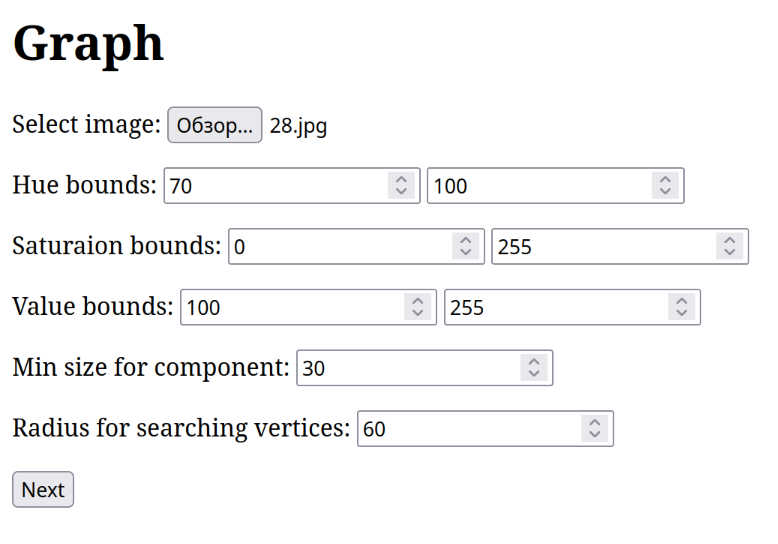
\includegraphics[width=\textwidth]{server1}
    \caption{Выбор изображения и параметров}
  \end{subfigure}
  \begin{subfigure}[b]{\textwidth}
    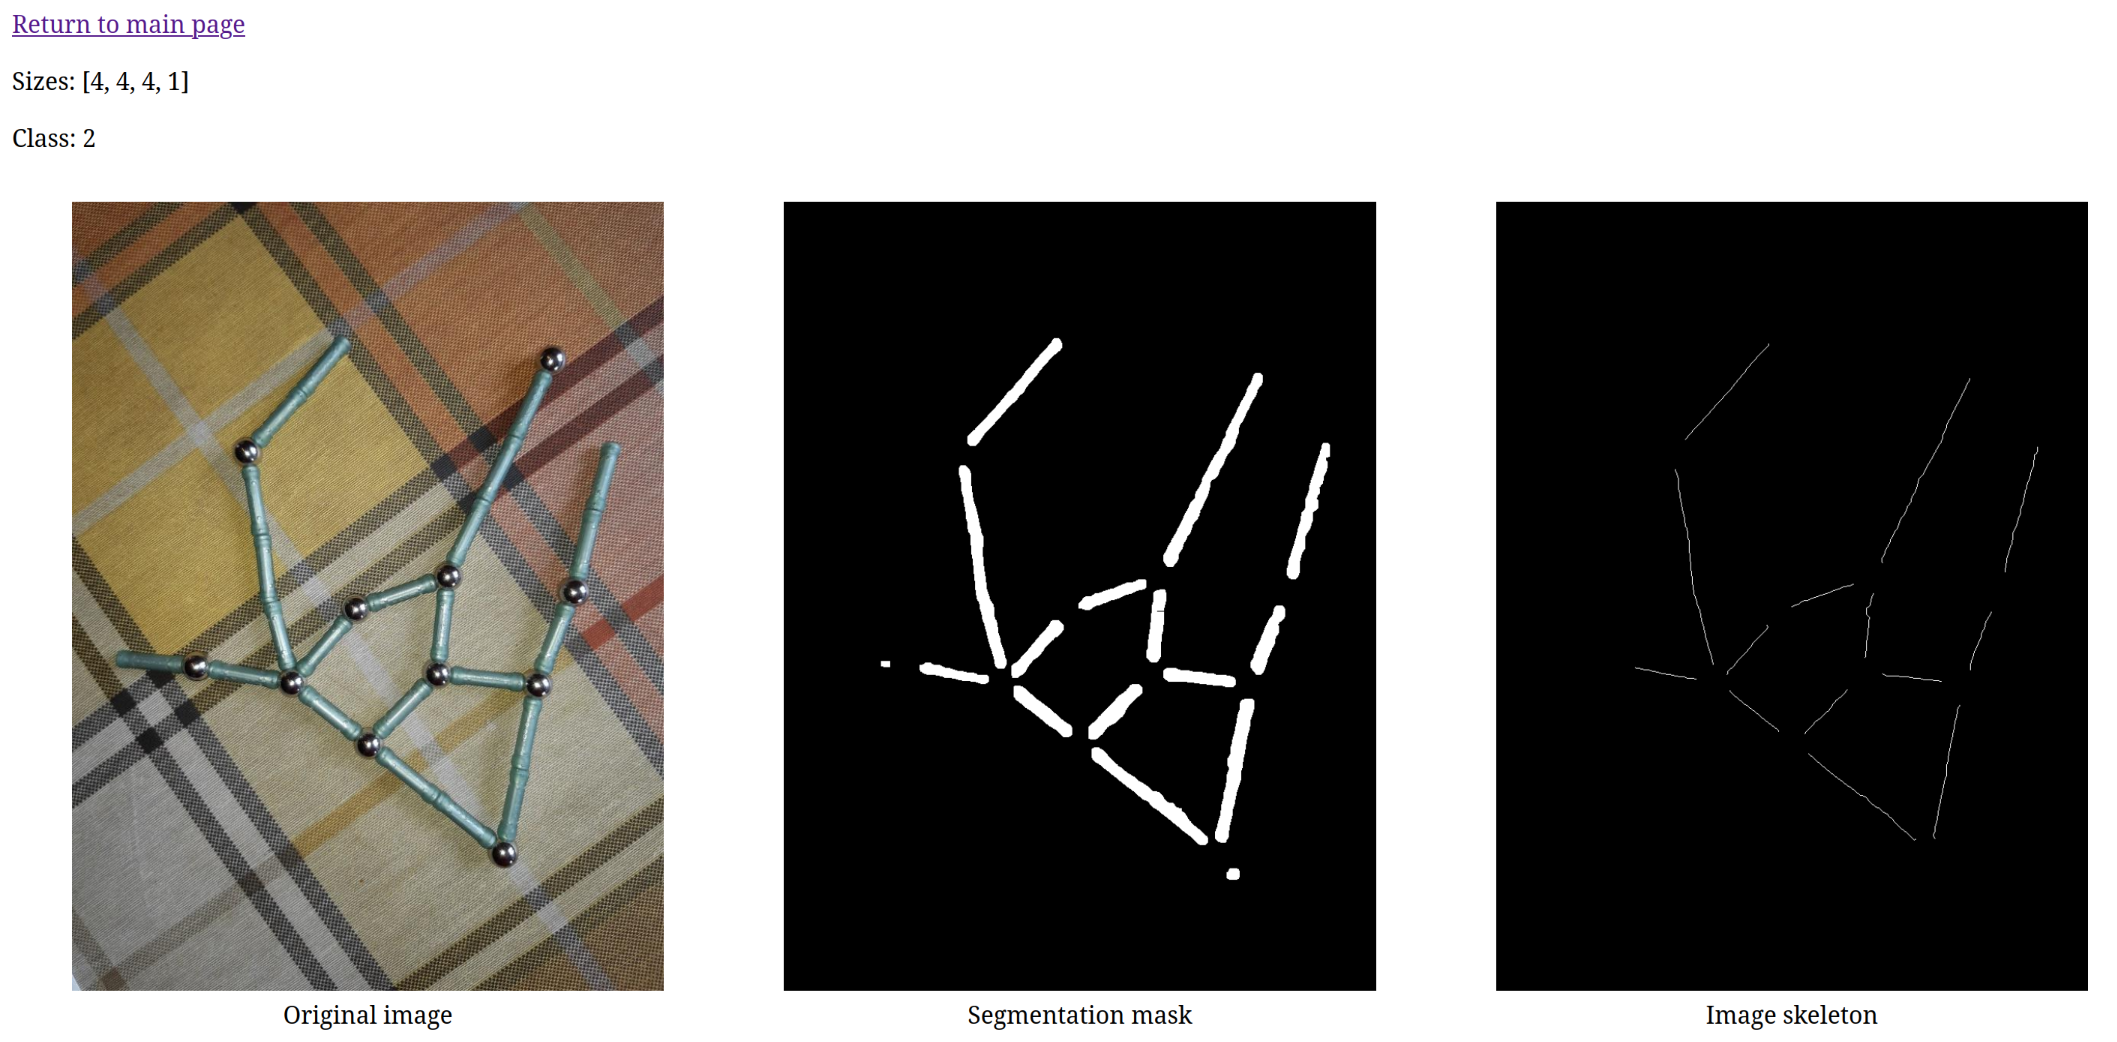
\includegraphics[width=\textwidth]{server2}
    \caption{Результат работы программы}
  \end{subfigure}
  \caption{Этапы работы с программой}
  \label{fig:program}
\end{figure}

\section{Описание программой реализации}
Программа была написана на языке программирования \verb|Python|. Для работы с изображениями использовалась библиотеки \verb|OpenCV| и \verb|scikit-image|.  Интерфейс был реализован в виде веб-сервера с помощью библиотеки \verb|Flask|. Для удобство решение было обернуто в docker-контейнер, однако возможна установка программы и всех зависимостей вручную.

Работа с программой происходит следующим образом (см. \autoref{fig:program}): сначала пользователь выбирает изображение для обработки и задает параметры программы.
Далее происходит выдача результата в виде маски сегментации исходного изображения, скелета изображения, признакового описания графа и результата классификации.

\section{Эксперименты}

Алгоритм хорошо себя показал на большинстве изображений, корректно составил бинаризованную маску, построил скелет из отрезков, соответствующим ребрам графа и построил признаковое описание изображенного графа. Таким образом, удается получить правильный класс изображения.

Однако на некоторых изображениях алгоритм не смог справиться с задачей. В первую очередь этого связано с неправильной сегментацией. На изображениях с пестрым фоном цвет магнитной головоломки совпадает с цветом фона, из-за чего трудно сегментировать изображение по цветам. Из-за неправильной сегментации, на скелете изображения возникают лишние <<ребра>> и строится неверное признаковое представление, и, как следствие, происходит неправильная классификация. Решением данной проблемы может быть более тонкий подбор параметров сегментации под каждое изображение.

\begin{figure}[h]
  \centering
  \begin{subfigure}[b]{0.9\textwidth}
    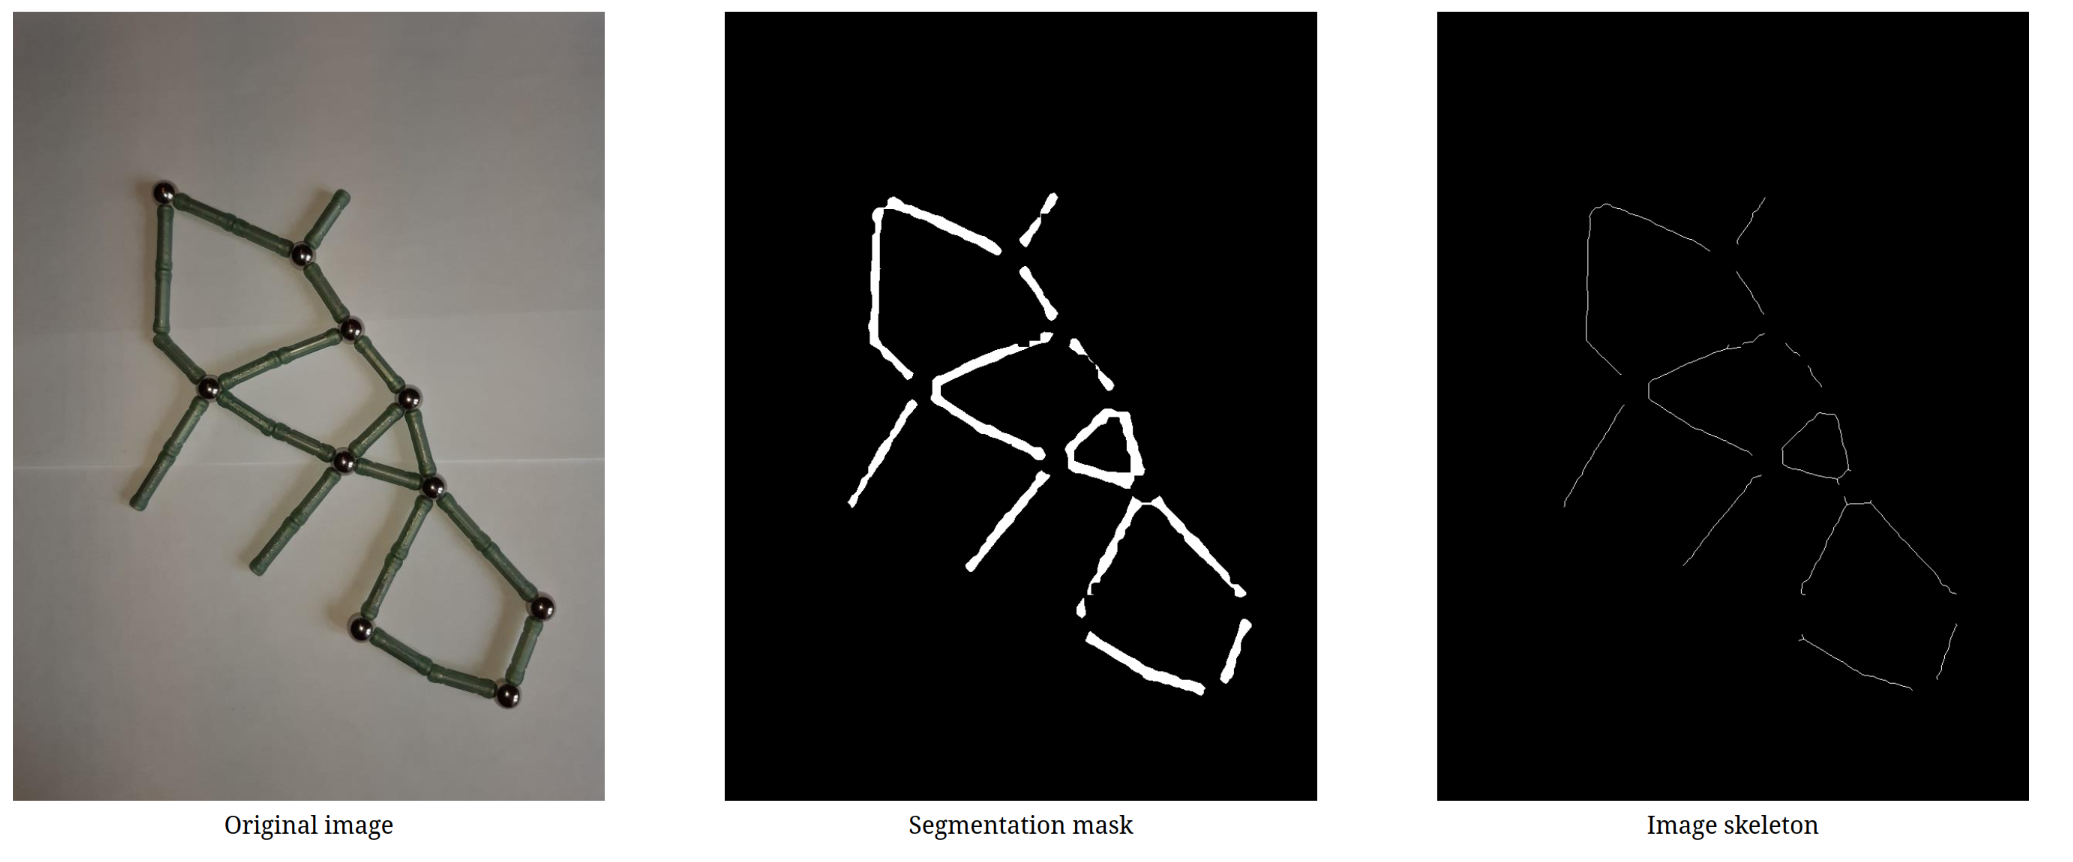
\includegraphics[width=\textwidth]{exp1}
    \caption{true label = 1, true vector = [3, 4, 3, 3] \\ pred label = 1, pred vector = [3, 4, 2, 1, 0, 0, 0, 0, 1]}
  \end{subfigure}
  \begin{subfigure}[b]{0.9\textwidth}
    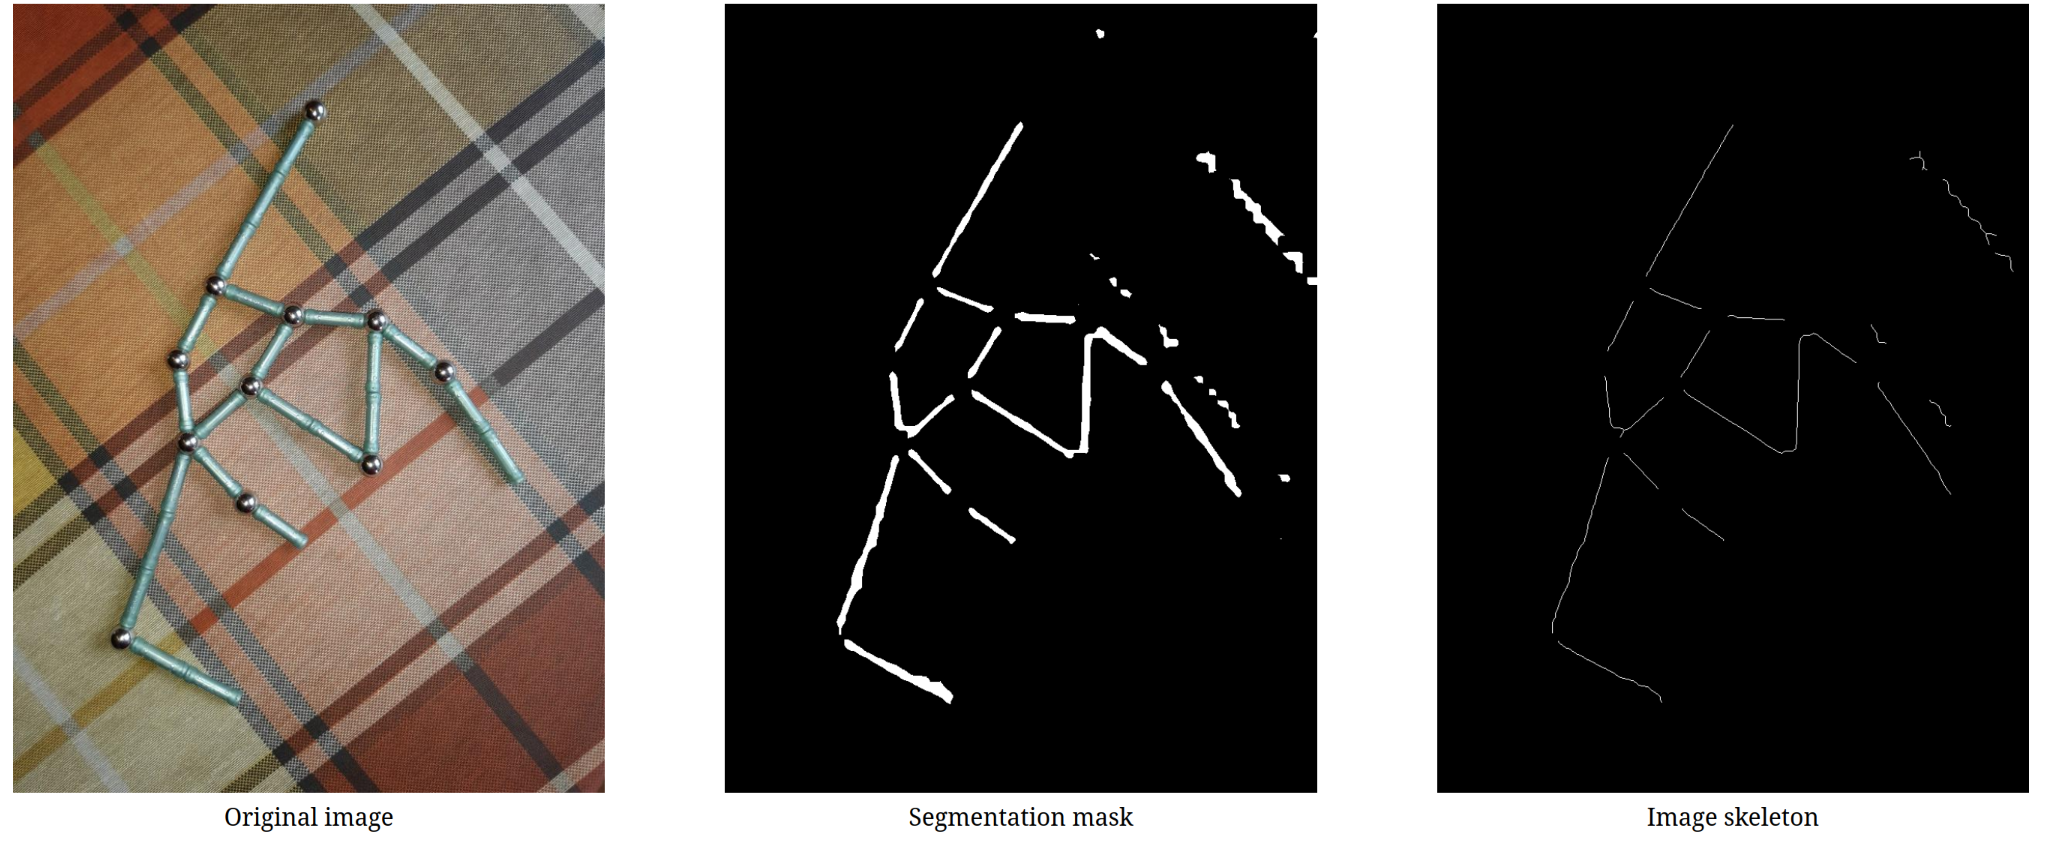
\includegraphics[width=\textwidth]{exp2}
    \caption{true label = 2, true vector = [4, 4, 4, 1], \\ pred label = 2, pred vector = [5, 4, 4, 2, 1]}
  \end{subfigure}
  \begin{subfigure}[b]{0.9\textwidth}
    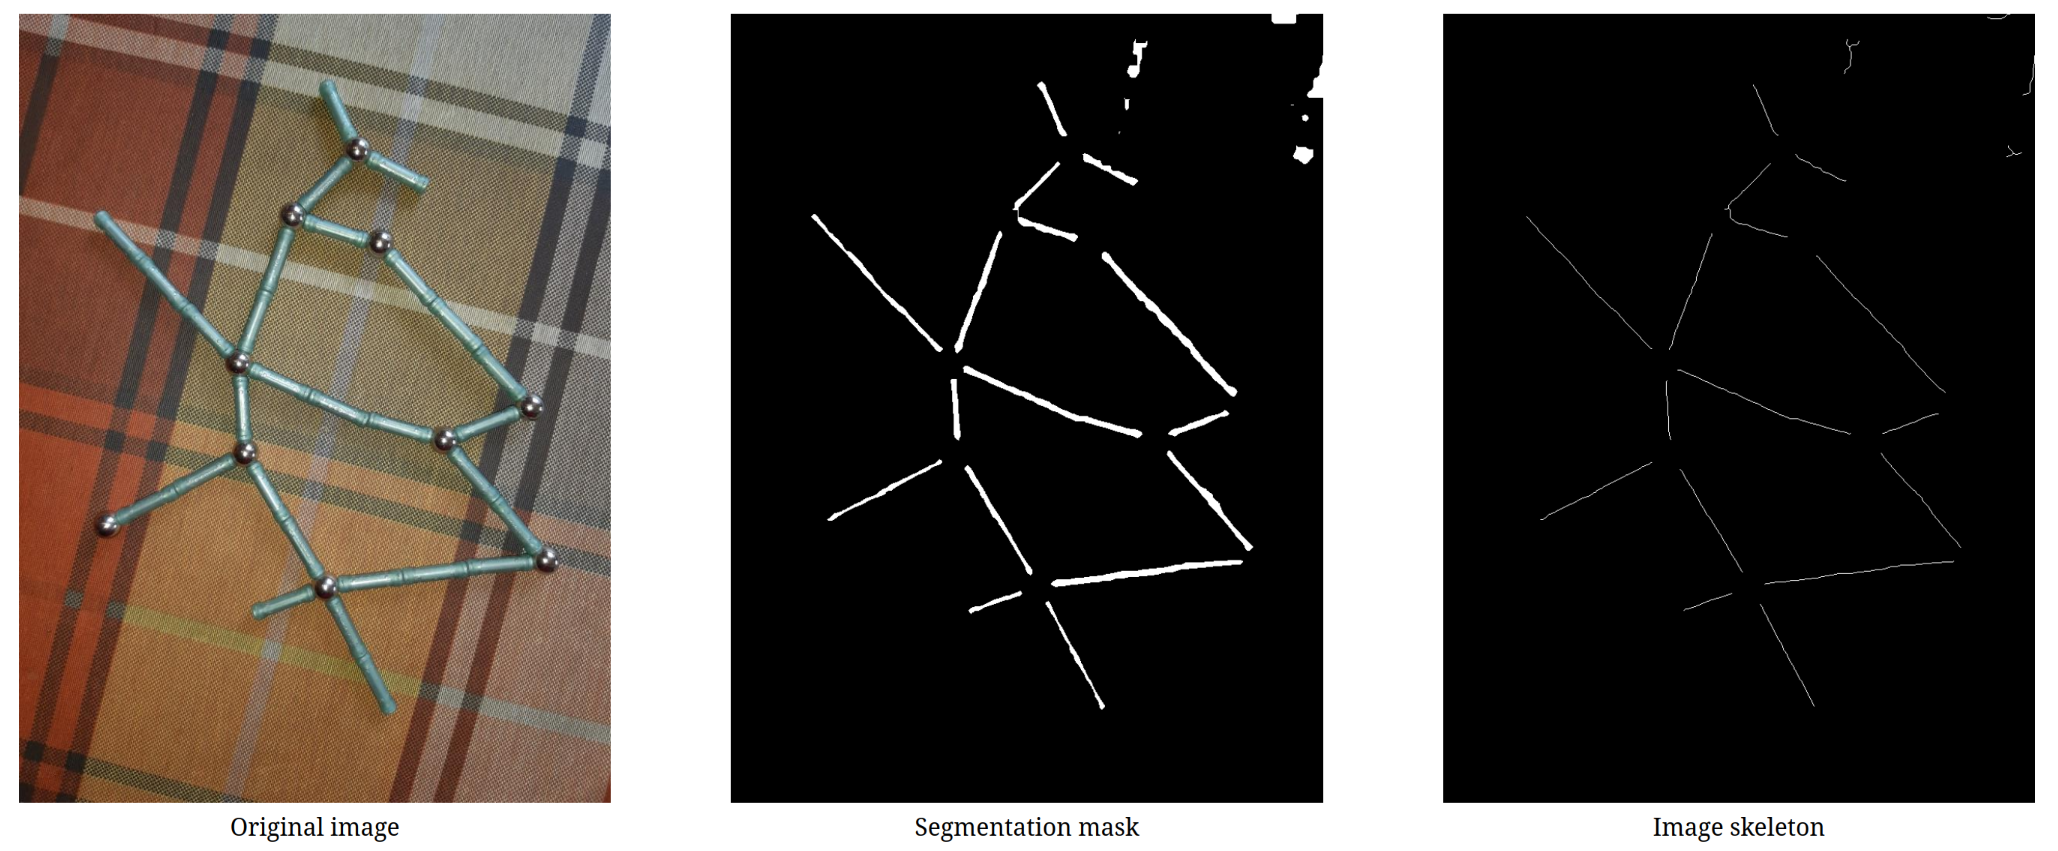
\includegraphics[width=\textwidth]{exp3}
    \caption{true label = 4, true vector = [6, 3, 3, 2] \\ pred label = 2, pred vector = [6, 6, 5, 2]}
  \end{subfigure}
  \caption{Эксперименты}
  \label{fig:exp}
\end{figure}


\section{Выводы}
Предложенный алгоритм смог добиться высокой точности при построении признакового описания графов и классификации изображений. Однако на изображениях с неоднородным фоном требуется точная настройка параметров для улучшения качества сегментации.

\end{document}